%----------------------------------------------------------------------------
\appendix
%----------------------------------------------------------------------------
\chapter*{\fuggelek}\addcontentsline{toc}{chapter}{\fuggelek}
\setcounter{chapter}{\appendixnumber}
%\setcounter{equation}{0} % a fofejezet-szamlalo az angol ABC 6. betuje (F) lesz
\numberwithin{equation}{section}
\numberwithin{figure}{section}
\numberwithin{lstlisting}{section}
%\numberwithin{tabular}{section}



%----------------------------------------------------------------------------
\section{Példa 1}
\label{sec:example1}
%----------------------------------------------------------------------------

\begin{figure}[h]
\small
\begin{verbatim}
S! -> S_NP_S_BAR(NP, S_BAR)
[tree] @(?2,?1)

S_BAR -> S_NP_VP(VP, PUNCT)
[tree] S3( *, ?1, ?2)

VP -> VP_VB_NP(VB,NP)
[tree] VP2(?1,?2)

NP -> NP_NN(NN)
[tree] NP1(?1)


NN -> John_NNP
[tree] NNP(John)

NN -> Mary_NNP
[tree] NNP(Mary)

VB -> loves_VBZ
[tree] VBZ(loves)

PUNCT -> punct_PUNCT
[tree] .(.)
\end{verbatim}
\caption{Egyszerű IRTG a \textit{John Loves Mary.} mondat TT-jének generálására}
\label{cod:example1}
\end{figure}

\begin{figure}[h]
\centering
\graphicspath{./}
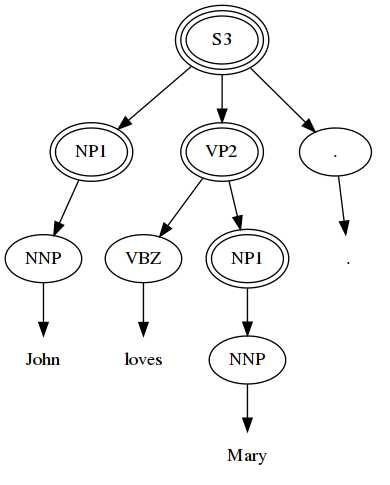
\includegraphics[scale=0.5]{figures/dots/example1.png}
\caption{~\ref{sec:example1}-ben leírt IRTG által generált levezetési fa a \textit{John Loves Mary.} mondat TT-jére.}
\label{fig:example1}
\end{figure}

\begin{figure}[h]
\small
\begin{verbatim}
@(
	S3( *, VP2( VBZ( loves ),  NP1( NNP( Mary ) ) ), .( . ) ), 
	NP1( NNP( John ) ) 
)
\end{verbatim}
\caption{~\ref{sec:example1}-ben leírt IRTG tree interpretációjának kimenete \textit{John Loves Mary.} mondat TT-jére.}
\label{cod:example1output}
\end{figure}

\clearpage

%----------------------------------------------------------------------------
\section{Példa 2}
\label{sec:example2}
%----------------------------------------------------------------------------

\begin{figure}[h!]
\small
\begin{verbatim}
S! -> NP( DT, JJ, NN )
[tree] NP3(?1,?2,?3)

DT -> the_DT
[tree] DT(the)

JJ -> black_JJ
[tree] NN(black)

VB -> cat_VB
[tree] VB(cat)
\end{verbatim}
\caption{Egyszerű három bemenetű IRTG a \textit{the black cat} szószerkezet TT-jének generálására}
\label{cod:example2}
\end{figure}

\begin{figure}[h]
\centering
\graphicspath{./}
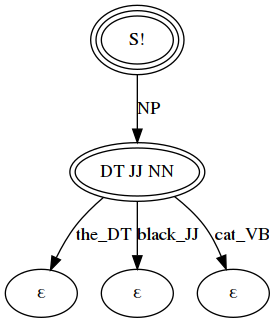
\includegraphics[scale=0.5]{figures/dots/example2.png}
\caption{~\ref{sec:example2}-ben leírt IRTG által generált levezetési fa a \textit{the black cat} szószerkezet TT-jére.}
\label{fig:example2}
\end{figure}

\begin{figure}[h]
\small
\begin{verbatim}
NP3( DT( the ), JJ( black ), NN( cat ) )
\end{verbatim}
\caption{~\ref{sec:example2}-ben leírt IRTG tree interpretációjának kimenete \textit{the black cat} szószerkezet TT-jére. A kimenet maga a \textit{the black cat} szószerkezet TT-je. }
\label{cod:example2output}
\end{figure}


\clearpage

%----------------------------------------------------------------------------
\section{Példa 3}
\label{sec:example3}
%----------------------------------------------------------------------------

\begin{figure}[h]
\small
\begin{verbatim}
S! -> NP_DT_NP_BAR( DT, NP_BAR)
[tree] @(?2,?1)

NP_BAR -> NP_BAR_JJ_NN(JJ,NN)
[tree] NP3(*,?1,?2)

DT -> the_DT
[tree] DT(the)

JJ -> black_JJ
[tree] NN(black)

VB -> cat_VB
[tree] VB(cat)
\end{verbatim}
\caption{Egyszerű IRTG a \textit{the black cat} szószerkezet TT-jének generálására}
\label{cod:example3}
\end{figure}

\begin{figure}[h]
\centering
\graphicspath{./}
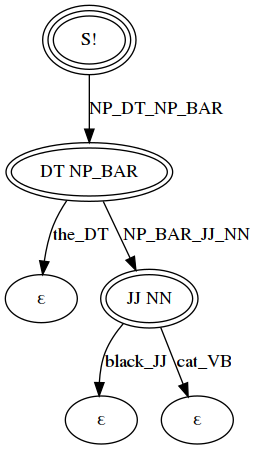
\includegraphics[scale=0.5]{figures/dots/example3.png}
\caption{~\ref{sec:example3}-ban leírt IRTG által generált levezetési fa a \textit{the black cat} szószerkezet TT-jére.}
\label{fig:example3}
\end{figure}

\begin{figure}[h!]
\begin{verbatim}
@(  NP3( *, JJ( black ), NN( cat ) ), DT( the ) )
\end{verbatim}
\caption{~\ref{sec:example3}-ben leírt IRTG tree interpretációjának kimenete a \textit{the black cat} szószerkezet TT-jére.}
\label{cod:example3output}
\end{figure}


\clearpage

%----------------------------------------------------------------------------
\section{Példa 4}
\label{sec:example4}
%----------------------------------------------------------------------------

\begin{figure}[h]
\small
\begin{verbatim}
S! -> NP_DT_NP_BAR( DT, NP_BAR)
[tree] @(?2,?1)

NP_BAR -> NP_BAR_JJ_NP_BAR(JJ,NP_BAR)
[tree] @(?2,?1)

NP_BAR -> NP_BAR_JJ_NN(JJ,NN)
[tree] NP4(* ,* ,?1 ,?2)

DT -> this_DT
[tree] DT(this)

JJ -> British_JJ
[tree] JJ(British)

JJ -> industrial_JJ
[tree] JJ(industrial)

NN -> conglomerate_NN
[tree] NN(conglomerate)
\end{verbatim}
\caption{Egyszerű IRTG a \textit{this British industrial conglomerate} szószerkezet TT-jének generálására}
\label{cod:example4}
\end{figure}

\begin{figure}[h!]
\centering
\graphicspath{./}
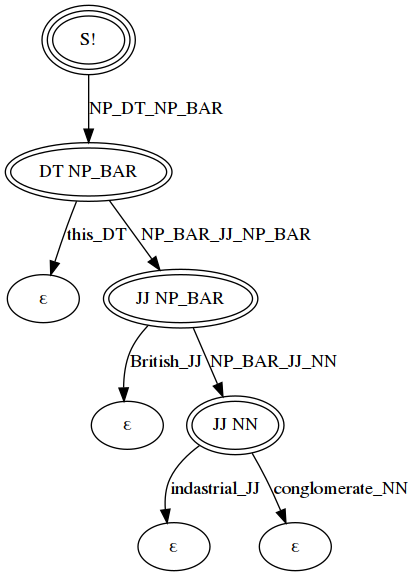
\includegraphics[scale=0.5]{figures/dots/example4.png}
\caption{~\ref{sec:example4}-ben leírt IRTG által generált levezetési fa a \textit{this British industrial conglomerate} szószerkezet TT-jére.}
\label{fig:example4}
\end{figure}


\clearpage

%----------------------------------------------------------------------------
\section{Példa 5}
\label{sec:example5}
%----------------------------------------------------------------------------

\begin{figure}[h]
\small
\begin{verbatim}
S! -> root_nsubj_NP_S_BAR(NP, S_BAR)
[ud] merge(
			f_dep(merge("(Root/Root :root r<root> :nsubj (d<dep>))", r_dep(?1))),
	 		?2
	 		)

S_BAR -> S_BAR_VP_PUNCT(VP, PUNCT)
[ud] ?1

VP -> dobj_VB_NP(VB,NP)
[ud] merge(f_dep(merge("(r<root> :dobj (d<dep>))", r_dep(?2))),?1)

NP -> NP_NN(NN)
[ud] ?1


NN -> John_NNP
[ud] "(John<root> / John)"

NN -> Mary_NNP
[ud] "(Mary<root> / Mary)"

VB -> loves_VBZ
[ud] "(loves<root> / loves)"

PUNCT -> punct_PUNCT
[ud] "(punct<root> / punct)"
\end{verbatim}
\caption{Egyszerű IRTG a \textit{John Loves Mary.} mondat UD gráfjának generálására}
\label{cod:example5}
\end{figure}

\begin{figure}[h]
\centering
\graphicspath{./}
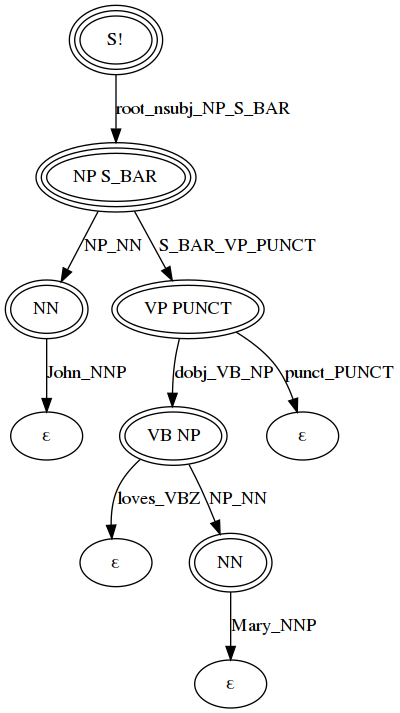
\includegraphics[scale=0.5]{figures/dots/example5_1.png}
\caption{~\ref{sec:example5}-ben leírt IRTG által generált levezetési fa a \textit{John loves Mary.} szószerkezet UD gráfját leíró s-graph-ra}
\label{fig:example5.1}
\end{figure}

\begin{figure}[h]
\small
\begin{verbatim}
merge(
	f_dep( merge(
		"(Root/Root :root r<root> :nsubj (d<dep>))",
 		r_dep( "(John<root> / John)" )
		) ),
	 merge(
		f_dep( merge(
					"(r<root> :dobj (d<dep>))", 
					r_dep( "(Mary<root> / Mary)" )
					) ),
 		“(loves<root> / loves)”
		)
	)
\end{verbatim}
\caption{~\ref{sec:example5} UD interpretációjának kimenete}
\label{fig:example5ud}
\end{figure}

\begin{figure}[h]
\centering
\graphicspath{./}
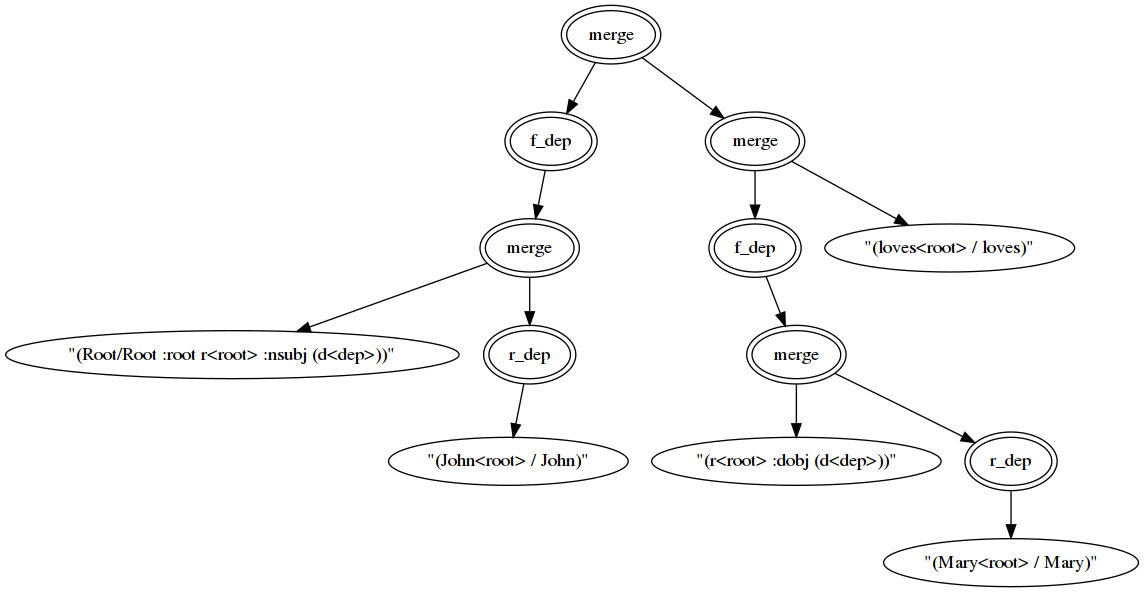
\includegraphics[scale=0.4]{figures/dots/example5_2.png}
\caption{~\ref{sec:example5}-ben leírt IRTG UD interpretációja által generált s-graph kifejezés műveleti fája}
\label{fig:example5.2}
\end{figure}

\begin{figure}[h]
\centering
\graphicspath{./}
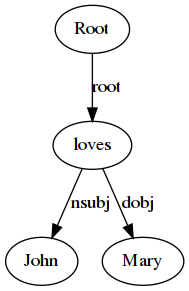
\includegraphics[scale=0.5]{figures/dots/example5_3.png}
\caption{~\ref{sec:example5}-ben leírt IRTG UD interpretációja által generált s-graph kifejezés végeredménye.
		Ez SGA formátumában így néz ki: "(Root/Root :root loves<root>/loves :nsubj (John/John) :dobj (Mary/Mary))"}
\label{fig:example5.3}
\end{figure}


\clearpage

%----------------------------------------------------------------------------
\section{Példa 6}
\label{sec:example6}
%----------------------------------------------------------------------------

\begin{figure}[h!]
\footnotesize
\begin{verbatim}
S! -> root_nsubj_NP_S_BAR(NP, S_BAR)
[tree] @(?2,?1)
[ud] merge(
			f_dep(merge("(Root/Root :root r<root> :nsubj (d<dep>))", r_dep(?1))),
			?2
			)
[fourlang] merge(
				f_dep(merge("(Root/Root :root r<root> :1,0 (d<dep>))", r_dep(?1))),
				?2
				)

S_BAR -> S_NP_VP(VP, PUNCT)
[tree] S3( *, ?1, ?2)
[ud] ?1
[fourlang] ?1

VP -> dobj_VB_NP(VB,NP)
[tree] VP2(?1,?2)
[ud] merge(
			f_dep(merge("(r<root> :dobj (d<dep>))", r_dep(?2))),
			?1
			)
[fourlang] merge(
				f_dep(merge("(r<root> :2 (d<dep>))", r_dep(?2))),
				?1
				)

NP -> NP_NN(NN)
[tree] NP1(?1)
[ud] ?1
[fourlang] ?1

NN -> John_NNP
[tree] NNP(John)
[ud] "(John<root> / John)"
[fourlang] "(John<root> / John)"

NN -> Mary_NNP
[tree] NNP(Mary)
[ud] "(Mary<root> / Mary)"
[fourlang] "(Mary<root> / Mary)"

VB -> loves_VBZ
[tree] VBZ(loves)
[ud] "(loves<root> / loves)"
[fourlang] "(loves<root> / loves)"

PUNCT -> punct_PUNCT
[tree] .(.)
[ud] "(punct<root> / punct)"
[fourlang] "(punct<root> / punct)"
\end{verbatim}
\caption{IRTG három algebrával a \textit{John Loves Mary.} mondat szintaktikai fájának, UD gráfjának és 4lang gráfjának generálására}
\label{cod:example6}
\end{figure}

\begin{figure}[h]
\centering
\graphicspath{./}
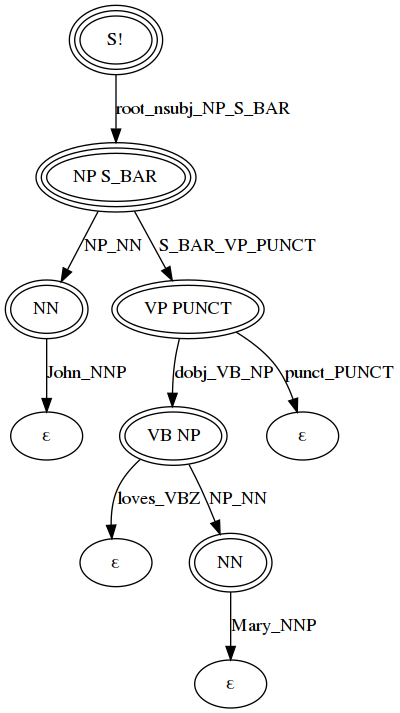
\includegraphics[scale=0.5]{figures/dots/example6_1.png}
\caption{~\ref{sec:example6}-ban leírt IRTG által generált levezetési fa a \textit{John loves Mary.} szószerkezet 4lang-ját leíró s-graph-ra}
\label{fig:example6}
\end{figure}

\begin{figure}[h]
\small
\begin{verbatim}
merge(
	f_dep( 
		merge(
			"(Root/Root :root r<root> :1,0 (d<dep>))",
 			r_dep( 
				"(John<root> / John)" 
				)
			) 
		),
 		merge(
			f_dep( 
					merge(
						"(r<root> :2 (d<dep>))", 
						r_dep( 
							"(Mary<root> / Mary)" 	
							)
						) 
				),
			 “(loves<root> / loves)”
			)
)
\end{verbatim}
\caption{~\ref{sec:example6} fourlang interpretációjának kimenete}
\label{fig:example6fourlang}
\end{figure}

\begin{figure}[h]
\centering
\graphicspath{./}
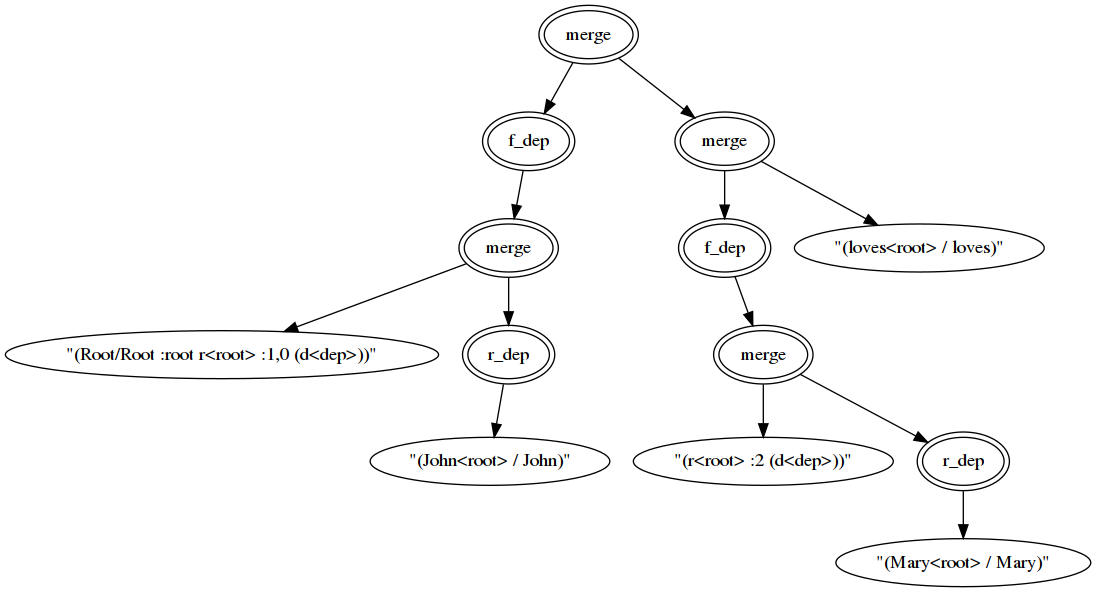
\includegraphics[scale=0.4]{figures/dots/example6_2.png}
\caption{~\ref{sec:example6}-ben leírt IRTG fourlang interpretációja által generált s-graph kifejezés műveleti fája}
\label{fig:example6.2}
\end{figure}

\begin{figure}[h]
\centering
\graphicspath{./}
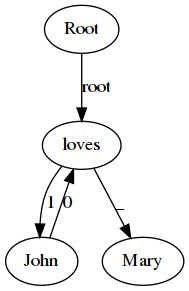
\includegraphics[scale=0.5]{figures/dots/example6_3.png}
\caption{~\ref{sec:example6}-ben leírt IRTG fourlang interpretációja által generált s-graph kifejezés végeredménye}
\label{fig:example6.3}
\end{figure}


\clearpage

%----------------------------------------------------------------------------
\section{Példa 7}
\label{sec:example7}
%----------------------------------------------------------------------------

\begin{figure}[h]
\small
\begin{verbatim}
//merge start
@(																				
	//merge start
	@(																			
		//graph1
		"( [ Root | | Root ] <root- ( [ r | root ] <nsubj- [ d | dep ] ) )",	
		//graph2
	 	"( [ John | root | John ] )",
	 	//tag of graph1
		dep,							
		//tag of graph2
		root,						
		//tag to forget	
		dep							
	//merge end
	),								
	//merge start
 	@(								
 		//merge start
		@(							
			//graph1
			"([ r | root ] <dobj- [ d | dep ] )", 		
			//graph2	
			"( [ Mary | root | Mary] )",
			//tag of graph1				
			dep,						
			//tag of graph2
			root,					
			//tag to forget	
			dep						
		//merge end
		) ,							
		//graph2
		“( [ loves | root | loves ] )”
	//megre end					
	)								
//merge end
)									
\end{verbatim}
\caption{Példakód az SGA fejlesztésével kapcsolatos koncepció szemléltetésére.
			A példa a \textit{John loves Mary.} mondat UD-gráfjára adott kimenetet dolgozza fel az új szintaxissal.}
\label{cod:example7}
\end{figure}

\clearpage

%----------------------------------------------------------------------------
\section{Példa 8}
\label{sec:example8}
%----------------------------------------------------------------------------

\begin{figure}[h]
\small
\begin{verbatim}
//merge the root of the left graph with root of the right graph
( 
//merge the dep of left graph with the root of the right graph, then we forget dep
( "( [ Root | | Root ] <root- ( [ r | root ] <nsubj- [ d | dep ] ) )" 
>dep@root< 
"( [ John | root | John ] )" X dep ) 

>root@root<

//merge the root of the left graph with root of the right graph
( 

//merge the dep of left graph with the root of the right graph, then we forget dep
( "([ r | root ] <dobj- [ d | dep ] )" 
>dep@root< 	//merge on dep of left graph and root of right graph
"( [ Mary | root | Mary ]  )" X	dep ) 

>root@root<	//merge on root of left graph and root of right graph

“( [ loves | root | loves ]  )” )

)
\end{verbatim}
\caption{Példakód az SGA operátoros verziójával kapcsolatos koncepció szemléltetésére.
			A példa a \textit{John loves Mary.} mondat UD-gráfjára adott kimenetet dolgozza fel az új szintaxissal.}
\label{cod:example8}
\end{figure}
